\chapter{Casing the Establishment}
\thispagestyle{plain}



\newacronym{iaaas}{IAAAS}{It’s All About Anonymity, Stupid}
\newacronym{Tor}{Tor}{The Onion Router}
\newacronym{ICANN}{ICANN}{Internet Corporation for Assigned
Names and Numbers}

\section{Hackers tools}

\emph{\gls{iaaas}}

Hackers use a wide variety of tools:
\begin{itemize}
    \item \emph{\gls{Tor}}, wich uses Layered cryptography with SOCKS proxy and Anonymous outgoing TCP connections
    \item Tor GUI client (Vidalia) and Privoxy (web filtering proxy)
    \item Google on browser for juicy targets
    \item tor-resolve instead of host for IP addresses
    \item proxychains to force connections through Tor and Nmap to scan service on targets
    \item socat to relay persistently, netcat to send requests to servers
\end{itemize}

\subsection{\emph{\gls{Tor}}}
How it works: 
\begin{enumerate}
    \item Alice \emph{\gls{Tor}} client obtain a list of \emph{\gls{Tor}} nodes from a directory server
    \item Alice \emph{\gls{Tor}} client picks a random path trough the nodes to the destination, using encrypted links
\end{enumerate}
\begin{figure}[H]
    \centering
    \begin{minipage}{0.48\textwidth}
        \centering
        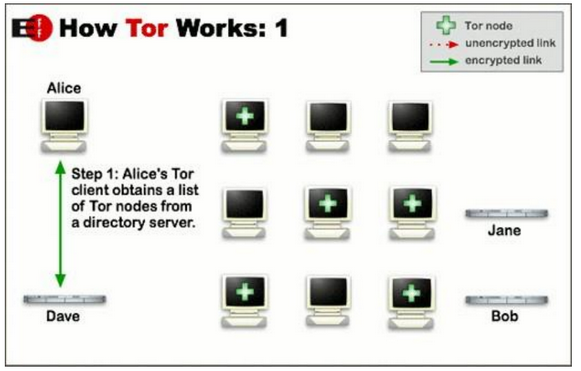
\includegraphics[width=\linewidth]{Include/Chapters/tor1.PNG}
        \caption{first step}\label{fig:img1}
    \end{minipage}
    \hfill
    \begin{minipage}{0.48\textwidth}
        \centering
        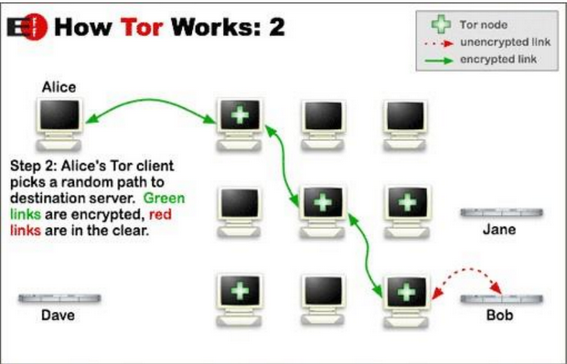
\includegraphics[width=\linewidth]{Include/Chapters/tor2.PNG}
        \caption{second step}
        \label{fig:img2}
    \end{minipage}
\end{figure}


\subsection{Vidalia}
Vidalia is a discontinued cross-platform GUI for controlling Tor.
It allows the user to start, stop or view the status of Tor

\subsection{Privoxy}
Privoxy is a free web proxy for enhancing
privacy, manipulating cookies and
modifying web page data and HTTP headers
before the page is rendered by the browser.
E.g.\ filtering web pages and removing
advertisements. Privoxy can be customized by
users.

\section{Footprinting}
What is footprinting? its the profiling of the target organization. It has to be done to give a picture of what the hacker can see. It has to be done regularly to minimize info leaks and implement monitoring

The profiling comprehend: 
\begin{itemize}
    \item Internet: domain names, network blocks and subnets, IP, TCP/UDP services, access controll, IDS, DNS hostnames, CPU arch, system enumeration
    \item intranet: network protocols, intranet domain names, network blocks, IP, TCP/UDP services
    \item Remote access: phone numbers, remote system type, VPN, authentication mechanism
    \item Extranet: domain names, connection source and destination, access control, type of connection
\end{itemize}

Profiling steps:
\begin{enumerate}
    \item Determine the scope of the activities
    \item get proper authorization trough politics and founding
    \item use publicly available information
    \item WHOIS and DNS enumeration: Domain names, IP addresses, port numbers
    \item DNS interrogation: obtain info about the organization by querying DNS server, DNS zone transfer by untrusted users. Use nslookup to map all resource records. Search with grep,sed,awk,perl
    \item network reconnaissance: topology and access path diagram using traceroute, tracert, visualroute, McAfee’s
NeoTrace, Foundstone’s Trout, Owasp
AMASS

\end{enumerate}

\subsection{publicly available information}
There are a lot of information on the internet that we can use:
\begin{itemize}
    \item HTML source code: using website mirroring tool for offline viewing, and reading things inside comment tags
    \item Enumerate hidden files and directories
    \item remote access to internal resources via browser: proxy to internal service
    \item looking for other website other than the main (web, test, VPN sites)
    \item related organization, to do a social engeneering attack or, in outsourced web developement, partners might not be as secure
    \item location details such as images or geolocalization: needed for surveillance, social engeneering, unauthorized access
    \item names: usernames, e-mail addresses
    \item phone number, phisical addresses
    \item employees personal details: home phone number, address, social security number, credit history, family ancestry, photos
    \item busness directory services
    \item job posting and resumes, ex employees
    \item employee home computers, for remote access to target, keystroke logger to see the passwords
    \item company history: mergers, acquisitions, scandals, layoff, hiring, reorganization, outsourcing, temorary contractors, business info, stock market sites
    \item privacy and security policies
    \item archived information
\end{itemize}

\subsection{Public Database Security Countermeasures}
A lot of countermeasures can be taken to minimize the leakage of data:
\begin{itemize}
    \item keeping administrative contacts up to date
    \item anonymize administrative contacts
    \item authenticate updates rigidly
    \item restrict zone transfer to only authorized servers
    \item Configure a firewall to deny unauthorized connection to TCP port 53
    \item configure not to provide internal DNS info
    \item discourage the use of HINFO records
    \item use intrusion detection: snort,bro
    \item Configure border routers to limit ICMP and UDP traffic to specific systems
\end{itemize}


\chapter{Scanning}
\section{Objectives}

\begin{enumerate}
    \item  determining if the system is alive
    \item determining which service are running or listening
    \item detecting operating system 
    \item Processing and storing data
\end{enumerate}


\section{Determining if the system is alive}
\subsection{same subnet}
Using ping sweeps: we can use ARP-SCAN, Nmap, Cain.
NMAP sends an ICMP ECHO request and ARP ping and TCP ping. If the target network is monitored by in IDS you could trigger an alert for the extra traffic generated

\subsection{remote host/router}
For a remote host we can use ICMP ECHO REQUEST, ICMP ECHO REPLY,ICMP TIMESTAMP,ICMP ADDRESS MASK
Others useful tools are: ping, nmap, hping3, nping, Superscan

\subsection{TCP/UDP host discovery}
When internal or external ICMP is not permitted.
For servers we use TCP/UDP service ports, for desktop we use local firewall trough remote desktop

\subsection{Ping sweep countermeasures}
Two type of countermeasures:
\begin{itemize}
    \item Detection: using IDS, commercial firewalls and host based tools like Scanlogd, courtney, ippl, protolog
    \item Prevention: using ACL in firewall to limit ICMP traffic in the network or system, allowing only ECHO REPLY, HOST UNREACHABLE, PROTOCOL UNREACHABLE, PORT UNREACHABLE, TIMESTAMP EXCEEDED only in specific host in DMZ. Allow only ISP's specific IP addresses
\end{itemize}

\section{determining which service are running or listening}
\subsection{Port scanning}
Port scanning has the objective to:
\begin{itemize}
    \item identify TCP/UDP services running on the target host
    \item identify the type of OS of the target
    \item identify application or version of the service
\end{itemize}

There are different types of port scanning:
\begin{itemize}
    \item TCP connect scan(3 way handshake)
    \item TCP SYN scan (half open scan)
    \item TCP FIN scan
    \item TCP NULL scan
    \item TCP Xmas scan
    \item TCP ACK scan
    \item TCP Window scan
    \item TCP windows scan
    \item UDP scan
\end{itemize}

\section{Detecting the Operating System}
OS detection is useful info for vulnerability mapping.
There are different techniques for OS detection: banner grabbing: using FTP, SMTP, HTTP, POP.
Stack fingerprinting: using TCP/IP stack implementation, making guesses from available ports (windows and unix have OS specific ports)


\subsection{Countermeasures}
Two type of countermeasures:
\begin{itemize}
    \item Detection: using Snort, Scanlog, option set
    \item Prevention: changing unique stack charateristic(not recommended), using a secure proxy or firewall, Active Defense.
\end{itemize}

\section{Processing and storing data}
The efficency to manage scan data is the speeed of the attack, and the number of system compromised.
Metasploit offers a vast platform of tools payloads and exploits

\chapter{Enumeration}
\section{What is enumeration?}
The difference between scannin and enumeration is the level of intrusiveness, and enumeration active cnnection to system and directed query, while scannin is passive.
Enumerated info comprehend: User account names, misconfigured shared files, older software version with known vulnerabilities, and default accounts and passwords. 

\subsection{vulnerability scanners}
There are a lot of tools for vulnerability scanning:
\begin{itemize}
    \item Using database of known vulnerabilities
    \item free scanners like: Nessus, OpenVAS
    \item Nessus provides a lot of tools, like: exhaustive scanning, custom plug ins, open source. Nessus countermeasures are: using IDS/IPS and audit yourself regularly.
\end{itemize}

\subsection{basic banner grabbing}
Banner grabbing is the process of analyze the banner of a service to obtain info about the software and version. The banner are the response messages of an open port.
It can be done manually using telnet, or automatically using netcat or nc.
The countermesure are: shutting down unecessary services, using an access control list, audit yourself regularly.

The most common services to grab are:
\begin{itemize}
    \item FTP, TCP 21: FTP password are sent in clear. The countermeasures are: using HTTP instead of FTP and disallow unresricted uploading
    \item Telnet, TCP 23: it has banners and alows bruteforce username enumeration. It sends password and data in cleartext. The countermeasures are: stop using telnet, or use a VPN, modify banner info, reconnect between failed login attempts.
    \item SMTP, TCP 25: SMTP can be enumerated with telnet using the commands VRFY (to confirm names of valid user) and EXPN (to reveal the actual delivery addresses of alias and mailing lists). The countermeasure is to disable EXPN and VRFY commands or restrict them to authenticated users 
    \item HTTP, TCP 80
    \item DNS, TCP/UDP 53: Zone transfer dump the entire contents of a domain's zone files. Its restricted to authorized machine on most DNS servers
    \item TFTP, UDP 69
    \item Finger, TCP 79
\end{itemize}

\subsection{DNS enumeration tools and countermeasures}
\begin{itemize}
    \item dnsenum: google scraping for additional subdomain, brute forcing subdomains, list domains network ranges, performs WHOIS on the ranges identified, Information correlation
    \item Fierce.pl 
\end{itemize}

The countemeasures are:
\begin{itemize}
    \item Using separate internal and externa DNS servers
    \item block or restrict DNS zone transfer
    \item restrict DNS queries to limit caache snooping 
\end{itemize}
\chapter{Hacking Windows and Rainbow Tables}
\section{}

\chapter{Cybercrime and Advanced Persistent Threats}
\section{}

\chapter{Remote Connectivity and VoIP Hacking}
\section{}

\chapter{Wireless Hacking}
\section{}

\chapter{Hacking Hardware}
\section{}

\chapter{Web Application Hacking}
\section{}

\chapter{Mobile Hacking}
\section{}